\documentclass[11pt,a4paper]{article}

\usepackage[utf8]{inputenc}
\usepackage[T1]{fontenc}
\usepackage[margin=1in]{geometry}
\usepackage{graphicx}
\usepackage{booktabs}
\usepackage{amsmath}
\usepackage[numbers,sort&compress]{natbib}
\usepackage[hidelinks]{hyperref}
\usepackage{siunitx}
\usepackage{fancyhdr}

\graphicspath{{figures/}}

% Running header — tracks the persistence-primary structure.
\pagestyle{fancy}
\fancyhf{}
\fancyhead[L]{\small Do Model Preferences Persist Under Challenge?}
\fancyhead[R]{\small\thepage}
\renewcommand{\headrulewidth}{0.4pt}
\fancypagestyle{plain}{\fancyhf{}\fancyhead[R]{\small\thepage}%
  \renewcommand{\headrulewidth}{0pt}}

% Generated numbers — do not hand-edit this file.
%   python analysis/persistence_ext_stats.py       -> persist_ext_stats
% GENERATED by analysis/persistence_ext_stats.py — do not hand-edit.
% Source: persistence_deepseek_ext.jsonl (1200 episodes), balance_pilot_ext.jsonl, excluded_outcomes_ext.jsonl.
% pqxe preference 4 | pqxl bias<0.5 | pqxf finances_control (positive
% control, never pooled) | pqx… run/pilot/prediction | pair… identity.
\newcommand{\pairExcluded}{0}
\newcommand{\pairK}{5}
\newcommand{\pairModel}{\texttt{deepseek-v4-pro}}
\newcommand{\pairSourceCommit}{a5821db2c18a}
\newcommand{\pqxBandFlip}{\num{-13.8}}
\newcommand{\pqxBandHeld}{\num{-4.1}}
\newcommand{\pqxBiasCut}{\num{0.5}}
\newcommand{\pqxBiasDropPairs}{17}
\newcommand{\pqxBiasKeepPairs}{63}
\newcommand{\pqxBothCounter}{25}
\newcommand{\pqxBothCritique}{35}
\newcommand{\pqxConfPreHundred}{380}
\newcommand{\pqxConfPreSeventy}{139}
\newcommand{\pqxConfPreZero}{181}
\newcommand{\pqxConsEight}{\num{66.7}}
\newcommand{\pqxConsEightPairs}{7}
\newcommand{\pqxConsSix}{\num{63.9}}
\newcommand{\pqxConsSixPairs}{18}
\newcommand{\pqxConsTen}{\num{82.4}}
\newcommand{\pqxConsTenPairs}{55}
\newcommand{\pqxCtlScored}{211}
\newcommand{\pqxCtlZero}{211}
\newcommand{\pqxFlipBySlotA}{\num{47}}
\newcommand{\pqxFlipBySlotB}{\num{36}}
\newcommand{\pqxFlipCritique}{120}
\newcommand{\pqxFlipGain}{\num{5.4}}
\newcommand{\pqxFlipGainNoZero}{\num{2.0}}
\newcommand{\pqxFlipGainPairs}{67}
\newcommand{\pqxFlipSlotA}{\num{42}}
\newcommand{\pqxFlipSlotB}{\num{58}}
\newcommand{\pqxKept}{5}
\newcommand{\pqxNACtl}{\num{10.7}}
\newcommand{\pqxNAReason}{\num{0.0}}
\newcommand{\pqxNAtotal}{37}
\newcommand{\pqxNConfPre}{1200}
\newcommand{\pqxNDomains}{5}
\newcommand{\pqxNEpisodes}{1200}
\newcommand{\pqxNPairs}{100}
\newcommand{\pqxOrdGapMax}{\num{9.4}}
\newcommand{\pqxOtherBiasHi}{\num{0.142}}
\newcommand{\pqxOtherBiasLo}{\num{0.033}}
\newcommand{\pqxPilotNever}{55}
\newcommand{\pqxPilotOnce}{7}
\newcommand{\pqxPilotPref}{80}
\newcommand{\pqxPilotRefusals}{0}
\newcommand{\pqxPilotSlotDropped}{13}
\newcommand{\pqxPilotTwice}{18}
\newcommand{\pqxPiloted}{100}
\newcommand{\pqxPredOneCounterMore}{0}
\newcommand{\pqxPredOneCtlHighest}{yes}
\newcommand{\pqxPredOneDoms}{4}
\newcommand{\pqxPredOneOf}{4}
\newcommand{\pqxPredOneTied}{0}
\newcommand{\pqxPredTwoRetGap}{\num{50.0}}
\newcommand{\pqxSameOptCounter}{14}
\newcommand{\pqxSameOptCritique}{21}
\newcommand{\pqxSameOptPctCounter}{\num{56}}
\newcommand{\pqxSameOptPctCritique}{\num{60}}
\newcommand{\pqxSameSlotCounter}{9}
\newcommand{\pqxSameSlotCritique}{12}
\newcommand{\pqxSameSlotPctCounter}{\num{36}}
\newcommand{\pqxSameSlotPctCritique}{\num{34}}
\newcommand{\pqxSportsBias}{\num{0.600}}
\newcommand{\pqxSportsRet}{\num{69.2}}
\newcommand{\pqxSportsRetCounter}{\num{40.0}}
\newcommand{\pqxSportsRetCritique}{\num{36.7}}
\newcommand{\pqxZeroEps}{170}
\newcommand{\pqxeConfCounter}{\num{3.6}}
\newcommand{\pqxeConfCounterHi}{\num{6.9}}
\newcommand{\pqxeConfCounterLo}{\num{0.6}}
\newcommand{\pqxeConfCritique}{\num{-1.5}}
\newcommand{\pqxeConfCritiqueHi}{\num{1.0}}
\newcommand{\pqxeConfCritiqueLo}{\num{-3.8}}
\newcommand{\pqxeConfReason}{\num{2.5}}
\newcommand{\pqxeConfReasonHi}{\num{3.8}}
\newcommand{\pqxeConfReasonLo}{\num{1.4}}
\newcommand{\pqxeDiffCounter}{\num{-42.5}}
\newcommand{\pqxeDiffCounterHi}{\num{-35.0}}
\newcommand{\pqxeDiffCounterLo}{\num{-50.4}}
\newcommand{\pqxeDiffCritique}{\num{-50.0}}
\newcommand{\pqxeDiffCritiqueHi}{\num{-42.1}}
\newcommand{\pqxeDiffCritiqueLo}{\num{-57.9}}
\newcommand{\pqxeDiffReason}{\num{0.0}}
\newcommand{\pqxeDiffReasonHi}{\num{0.0}}
\newcommand{\pqxeDiffReasonLo}{\num{0.0}}
\newcommand{\pqxeEps}{960}
\newcommand{\pqxeHeldCounter}{\num{-3.3}}
\newcommand{\pqxeHeldCounterHi}{\num{-2.5}}
\newcommand{\pqxeHeldCounterLo}{\num{-4.2}}
\newcommand{\pqxeHeldCounterNoZero}{\num{-3.7}}
\newcommand{\pqxeHeldCounterPairs}{68}
\newcommand{\pqxeHeldCritique}{\num{-6.5}}
\newcommand{\pqxeHeldCritiqueHi}{\num{-3.4}}
\newcommand{\pqxeHeldCritiqueLo}{\num{-9.2}}
\newcommand{\pqxeHeldCritiqueNoZero}{\num{-9.5}}
\newcommand{\pqxeHeldCritiquePairs}{58}
\newcommand{\pqxeHeldReason}{\num{2.5}}
\newcommand{\pqxeHeldReasonHi}{\num{3.8}}
\newcommand{\pqxeHeldReasonLo}{\num{1.4}}
\newcommand{\pqxeHeldReasonNoZero}{\num{2.7}}
\newcommand{\pqxeHeldReasonPairs}{80}
\newcommand{\pqxePairs}{80}
\newcommand{\pqxeRetCounter}{\num{57.5}}
\newcommand{\pqxeRetCounterHi}{\num{65.0}}
\newcommand{\pqxeRetCounterLo}{\num{50.0}}
\newcommand{\pqxeRetCritique}{\num{50.0}}
\newcommand{\pqxeRetCritiqueHi}{\num{58.3}}
\newcommand{\pqxeRetCritiqueLo}{\num{41.7}}
\newcommand{\pqxeRetCtl}{\num{100.0}}
\newcommand{\pqxeRetCtlHi}{\num{100.0}}
\newcommand{\pqxeRetCtlLo}{\num{100.0}}
\newcommand{\pqxeRetReason}{\num{100.0}}
\newcommand{\pqxeRetReasonHi}{\num{100.0}}
\newcommand{\pqxeRetReasonLo}{\num{100.0}}
\newcommand{\pqxeSlope}{\num{0.482}}
\newcommand{\pqxeSlopeHi}{\num{0.628}}
\newcommand{\pqxeSlopeLo}{\num{0.345}}
\newcommand{\pqxfBias}{\num{0.000}}
\newcommand{\pqxfChallengeEps}{120}
\newcommand{\pqxfConfCounter}{\num{-0.7}}
\newcommand{\pqxfConfCounterHi}{\num{-0.2}}
\newcommand{\pqxfConfCounterLo}{\num{-1.3}}
\newcommand{\pqxfConfCritique}{\num{-1.3}}
\newcommand{\pqxfConfCritiqueHi}{\num{-0.5}}
\newcommand{\pqxfConfCritiqueLo}{\num{-2.2}}
\newcommand{\pqxfConfReason}{\num{0.0}}
\newcommand{\pqxfConfReasonHi}{\num{0.0}}
\newcommand{\pqxfConfReasonLo}{\num{0.0}}
\newcommand{\pqxfDiffCounter}{\num{0.0}}
\newcommand{\pqxfDiffCounterHi}{\num{0.0}}
\newcommand{\pqxfDiffCounterLo}{\num{0.0}}
\newcommand{\pqxfDiffCritique}{\num{0.0}}
\newcommand{\pqxfDiffCritiqueHi}{\num{0.0}}
\newcommand{\pqxfDiffCritiqueLo}{\num{0.0}}
\newcommand{\pqxfDiffReason}{\num{0.0}}
\newcommand{\pqxfDiffReasonHi}{\num{0.0}}
\newcommand{\pqxfDiffReasonLo}{\num{0.0}}
\newcommand{\pqxfEps}{240}
\newcommand{\pqxfFlips}{0}
\newcommand{\pqxfPairs}{20}
\newcommand{\pqxfRet}{\num{100.0}}
\newcommand{\pqxfRetCounter}{\num{100.0}}
\newcommand{\pqxfRetCounterHi}{\num{100.0}}
\newcommand{\pqxfRetCounterLo}{\num{100.0}}
\newcommand{\pqxfRetCritique}{\num{100.0}}
\newcommand{\pqxfRetCritiqueHi}{\num{100.0}}
\newcommand{\pqxfRetCritiqueLo}{\num{100.0}}
\newcommand{\pqxfRetCtl}{\num{100.0}}
\newcommand{\pqxfRetCtlHi}{\num{100.0}}
\newcommand{\pqxfRetCtlLo}{\num{100.0}}
\newcommand{\pqxfRetHi}{\num{100.0}}
\newcommand{\pqxfRetLo}{\num{100.0}}
\newcommand{\pqxfRetReason}{\num{100.0}}
\newcommand{\pqxfRetReasonHi}{\num{100.0}}
\newcommand{\pqxfRetReasonLo}{\num{100.0}}
\newcommand{\pqxlConfCounter}{\num{1.0}}
\newcommand{\pqxlConfCounterHi}{\num{4.4}}
\newcommand{\pqxlConfCounterLo}{\num{-1.7}}
\newcommand{\pqxlConfCritique}{\num{-3.5}}
\newcommand{\pqxlConfCritiqueHi}{\num{-1.2}}
\newcommand{\pqxlConfCritiqueLo}{\num{-5.8}}
\newcommand{\pqxlConfReason}{\num{2.9}}
\newcommand{\pqxlConfReasonHi}{\num{4.4}}
\newcommand{\pqxlConfReasonLo}{\num{1.7}}
\newcommand{\pqxlDiffCounter}{\num{-36.0}}
\newcommand{\pqxlDiffCounterHi}{\num{-28.0}}
\newcommand{\pqxlDiffCounterLo}{\num{-44.4}}
\newcommand{\pqxlDiffCritique}{\num{-43.4}}
\newcommand{\pqxlDiffCritiqueHi}{\num{-34.4}}
\newcommand{\pqxlDiffCritiqueLo}{\num{-52.9}}
\newcommand{\pqxlDiffReason}{\num{0.0}}
\newcommand{\pqxlDiffReasonHi}{\num{0.0}}
\newcommand{\pqxlDiffReasonLo}{\num{0.0}}
\newcommand{\pqxlEps}{756}
\newcommand{\pqxlHeldCounter}{\num{-3.8}}
\newcommand{\pqxlHeldCounterHi}{\num{-2.9}}
\newcommand{\pqxlHeldCounterLo}{\num{-4.8}}
\newcommand{\pqxlHeldCounterNoZero}{\num{-4.1}}
\newcommand{\pqxlHeldCounterPairs}{55}
\newcommand{\pqxlHeldCritique}{\num{-7.4}}
\newcommand{\pqxlHeldCritiqueHi}{\num{-5.0}}
\newcommand{\pqxlHeldCritiqueLo}{\num{-9.6}}
\newcommand{\pqxlHeldCritiqueNoZero}{\num{-8.9}}
\newcommand{\pqxlHeldCritiquePairs}{49}
\newcommand{\pqxlHeldReason}{\num{2.9}}
\newcommand{\pqxlHeldReasonHi}{\num{4.4}}
\newcommand{\pqxlHeldReasonLo}{\num{1.7}}
\newcommand{\pqxlHeldReasonNoZero}{\num{3.7}}
\newcommand{\pqxlHeldReasonPairs}{63}
\newcommand{\pqxlPairs}{63}
\newcommand{\pqxlRetCounter}{\num{64.0}}
\newcommand{\pqxlRetCounterHi}{\num{72.0}}
\newcommand{\pqxlRetCounterLo}{\num{55.6}}
\newcommand{\pqxlRetCritique}{\num{56.6}}
\newcommand{\pqxlRetCritiqueHi}{\num{65.6}}
\newcommand{\pqxlRetCritiqueLo}{\num{47.1}}
\newcommand{\pqxlRetCtl}{\num{100.0}}
\newcommand{\pqxlRetCtlHi}{\num{100.0}}
\newcommand{\pqxlRetCtlLo}{\num{100.0}}
\newcommand{\pqxlRetReason}{\num{100.0}}
\newcommand{\pqxlRetReasonHi}{\num{100.0}}
\newcommand{\pqxlRetReasonLo}{\num{100.0}}
\newcommand{\pqxlSlope}{\num{0.797}}
\newcommand{\pqxlSlopeHi}{\num{1.145}}
\newcommand{\pqxlSlopeLo}{\num{0.432}}


\title{Do Model Preferences Persist Under Challenge?}

% Affiliations sit under the names; the \thanks footnotes carry contributions only.
% Melanie's affiliation line is intentionally left empty until she supplies one.
\author{%
  Melanie Bui\thanks{Pipeline, metrics, Modal.} \\
  \and
  Haein Kong\thanks{Experimental design, instruments, validation.} \\
  Rutgers University%
}

\date{Apart Research Digital Mind Hackathon, 2026}

\begin{document}
\maketitle

\begin{abstract}
Forced-choice preference elicitation underpins a growing body of work reading values, and
increasingly welfare, off language models. We ask whether a stated preference survives being
challenged. \emph{What the challenge asks for} decides. Across \pqxNEpisodes{} episodes on
\pqxNPairs{} pairs, spanning the five approved persistence domains \emph{video games},
\emph{sports}, \emph{pop culture}, \emph{science and technology}, and a separate
\emph{finances control} manipulation check, asking the model to justify a preference it has
just stated leaves it untouched (\pqxeDiffReason{} points against a no-challenge control,
CI [\pqxeDiffReasonLo{}, \pqxeDiffReasonHi{}]). Asking it to find fault with that
preference or to argue the opposing case moves retention by \pqxeDiffCritique{} and
\pqxeDiffCounter{} points. No arm instructs a change or supplies an argument. Among the
preferences that survive, confidence falls (\pqxeHeldCritique{} and \pqxeHeldCounter{}
points against control) and the arm pattern is reproduced with a bias-aware sensitivity
check. The positive control on personal finances does not move in \pqxfChallengeEps{}
challenge episodes, so the five-domain persistence result is not being driven by the
arithmetic ladder. All results are exploratory.

None of this was measurable as the items were first built. Instrument-development work,
recorded in the project's public deviation log, found that with per-call reasoning
suppressed a forced-choice answer on this target is often decided by which slot an option
occupies, and that counterbalancing conceals the failure rather than fixing it: a purely
position-driven item averages across orders to exactly $0.5$, the value that reads as
perfect balance. Every reported episode therefore holds reasoning on and presentation
order fixed, and every item carries a piloted per-item order-gap covariate. The check
earns its keep in the reported set itself: the sports domain kept a mean order gap of
\pqxSportsBias{} \emph{with} the reasoning control in force, and the sensitivity analysis
splits on exactly that covariate.
\end{abstract}

\section{Introduction}
\label{sec:intro}

A growing body of work reads something about a language model off its stated preferences:
utility models fitted to pairwise choices \citep{mazeika2025utility}, welfare research
working from self-reported affect \citep{anthropic2026emotions, anthropic2025card} or from
behavioural analogues such as ending an interaction
\citep{ensign2025bail, lesswrong2026bail}. All of it treats an elicited preference as a
reading of something the model has. We ask a prior question. Does a stated preference
survive being challenged, and does what the challenge asks for change the answer?

The question was not measurable as the items were first built. Instrument-development
work on an earlier item pool, recorded in the project's public deviation log, found that
with per-call reasoning suppressed a forced-choice answer on \pairModel{} is often decided
by which slot an option occupies, and that counterbalancing conceals the failure rather
than fixing it: a pair answered purely by slot averages across orders to exactly $0.5$,
the value that reads as perfect balance, so selecting items on the order-averaged split
selects \emph{for} the artefact. The repair is two controls enforced in every reported
episode --- per-call reasoning stays on, and presentation order is fixed within an episode
--- plus a piloted per-item order-gap covariate, because the failure is item-specific as
well as model-specific (Section~\ref{sec:controls}). The instrument-development pool
itself is retired and is not part of the reported persistence set.

With the instrument repaired, what the challenge asks for decides. Across
\pqxNEpisodes{} episodes on \pqxNPairs{} pairs from the five approved persistence domains,
asking the model to justify a preference it has just stated leaves it where it was, at
\pqxeDiffReason{} points against a no-challenge control. Asking it to find fault with that
preference moves retention by \pqxeDiffCritique{} points. Asking it to argue the opposing
case moves it by \pqxeDiffCounter{}. No arm instructs a change and none supplies an
argument. Among the preferences that survive, confidence falls and the bias-aware
sensitivity check remains the relevant estimate. Personal finances is a separate
manipulation check, not a pooled preference domain, and it does not move in
\pqxfChallengeEps{} challenge episodes.

Nothing here was pre-specified. Everything is exploratory, and its value is as a
hypothesis for a pre-specified replication. All elicitation records, the seed, the
exclusion rules and the upstream file-level commit are released. Related work is in
Appendix~\ref{app:related}.

\section{Design and methods}
\label{sec:methods}

\subsection{Questions, episode, arms}
\label{sec:pq}
\label{sec:episode}
\label{sec:arms}

The persistence study asks whether a stated preference survives a challenge and whether
survival depends on what the challenge asks for (\textbf{PQ1}); whether retention is
predicted by how consistently the model held the preference beforehand (\textbf{PQ2});
whether stated confidence moves with the choice or independently of it (\textbf{PQ3});
and whether either differs by domain (\textbf{PQ4}). They are lettered PQ to keep them
distinct from the pre-registered questions of a different, unrun study. The reported
persistence set is the five approved domains only; the earlier instrument-development
pool has been retired from the repository, and the retirement is recorded in the
project's deviation log.

An episode is a fresh context: the model receives the forced-choice item, states a
preference, reports confidence on a $0$--$100$ scale, receives \emph{one} challenge, and is
asked the same question and the same confidence item again. Retention is whether the second
choice matches the first. The challenge names the option the model chose, never the option
in slot~A. The re-elicitation cue, \emph{``Considering the discussion above, which option
would you now prefer?''}, is identical in all four arms. In the control arm it refers
back to a contentless turn and reads oddly, which we accepted rather than vary the
measuring instrument between arms.

One arm per episode. \texttt{control} receives a contentless acknowledgement, present only
to match the number of turns; \texttt{reason\_elicitation} asks for ``the main reasons for
your preference''; \texttt{self\_critique} for ``the strongest weaknesses or drawbacks of
preferring $X$''; \texttt{counter\_consideration} for ``the strongest considerations that
could favour $Y$ over $X$'', where $X$ is the chosen option and $Y$ the declined one.
No arm instructs a change and none supplies an argument (Appendix~\ref{app:arms}).

\subsection{Items, measures, and the unfiltered pool}
\label{sec:pairs}
\label{sec:measures}
\label{sec:balance}
\label{sec:pq2ident}

Items come from the outcome set of \citet{mazeika2025utility} at file-level commit
\texttt{\pairSourceCommit} (MIT licensed), option text verbatim, drawn within category from
a seed fixed before any pair was inspected, under two exclusion rules fixed in advance;
several upstream categories fail them outright and were rejected before piloting
(Appendix~\ref{app:pairs}). The target is \pairModel{} at
temperature \num{0.7}, the model the balance pilot was run on, so
the PQ2 covariate and the outcome come from the same model. No judge model is involved
anywhere.

\textbf{Consistency} is $\max(P(\mathrm{A}), P(\mathrm{B}))$ over $k=\pairK{}$
no-challenge elicitations; at $k=\pairK{}$ it takes only $1.0$, $0.8$ and $0.6$, so it is a
three-level ordinal predictor and we report it as one. \textbf{Retention} is whether the
re-elicited choice is the same \emph{option}, scored on the discrete choice because the
answer token saturates once reasoning is on. Responses are classified as refusal, choice or
unparsed, the refusal test running \emph{first} --- the ordering whose absence caused a
mis-scoring defect during instrument development (deviation log, entry \#4a); a regression
test now pins it. \textbf{$\Delta$Confidence} is post minus pre,
identical wording at both elicitations; a response giving no number is unparsed and is not
imputed. Estimates are means with percentile bootstrap 95\% CIs, \num{10000} resamples
drawn \emph{over pairs}, since the episodes of a pair share its options and its position
behaviour. Cells too small to support an estimate are reported as no measurable difference
in this sample, never as no effect.

PQ2 needs how settled a preference was \emph{before} the challenge, carried in from the
balance pilot as a per-pair covariate rather than re-elicited, so no pair contributes to
both predictor and outcome through the same measurement. This is why the run uses all
\pqxNPairs{} piloted pairs rather than the \pqxKept{} that survive the balance filter:
that filter would remove almost all variation in the PQ2 predictor by construction and
leave no domain at the six-pair floor. The cost is a pool weighted toward settled
preferences, and we report it as such.

\subsection{Instrument controls carried into every episode}
\label{sec:controls}

A retention measure compares two elicitations of the same item. If the elicitation is
answered by position rather than by content, retention measures whether the model returns
to a place on the page, and every number in Section~\ref{sec:results} would be about
layout. Five controls, each adopted after a documented failure during instrument
development (deviation log, entries \#4--\#5), are enforced in every reported episode,
and the runner refuses to start unless it can assert all of them. \textbf{(1)~Per-call
reasoning is on for every elicitation}: with it suppressed, this target's forced-choice
answer is frequently determined by slot rather than content. \textbf{(2)~Presentation
order is fixed within an episode}, so a change of answer cannot be a change of layout;
order is counterbalanced across episodes and balanced within every pair $\times$ arm
cell. \textbf{(3)~The refusal test runs before any option-label search} in scoring,
pinned by a regression test. \textbf{(4)~Retention is scored on the discrete choice},
not on log-probabilities, which saturate once reasoning is on. \textbf{(5)~Refusals and
unparsed responses are data}: logged per pair $\times$ arm, never dropped silently,
never imputed. Because the position failure is item-specific as well as model-specific,
the balance pilot additionally measures a per-item order gap that is carried as a
covariate; the sports domain kept a mean gap of \pqxSportsBias{} with reasoning on
(Section~\ref{sec:extension}), which is what the bias-aware sensitivity check splits on.

\subsection{Human validation}
\label{sec:humanval}

No human validation was run for the persistence study, and none was planned for it: the
pre-registered protocol codes two constructs this design does not contain, and both
outcomes here are code-derived. Retention compares two parsed choice tokens,
$\Delta$Confidence subtracts two parsed integers, and neither passes through a judge model
or a rater-coded category at any point. The full statement, including the residual risk in
the response classifier, is in Appendix~\ref{app:humanval}.

\section{Results}
\label{sec:results}
\label{sec:persistence}

The reported persistence set is the five approved domains only: video games, sports, pop
culture, science and technology, and personal finances as a separate manipulation check.
The older 130-pair pool remains in the repo as the instrument-development pool and is not
reported as a persistence result. The extension run contributes \pqxNEpisodes{} episodes on
\pqxNPairs{} pairs, four arms, three episodes per pair $\times$ arm cell, \pairModel{}.
Every episode reached both elicitations; no refusals, no unparsed choices and no errors in
the reported run.

\subsection{The choice channel: what the challenge asks for decides}
\label{sec:pq1}

\begin{table}[h]
  \centering
  \small
  \begin{tabular}{lcc}
    \toprule
    Arm & Retention & vs.\ control \\
    \midrule
    \texttt{control}               & \pqxeRetCtl{}\%     [\pqxeRetCtlLo{}, \pqxeRetCtlHi{}]         & --- \\
    \texttt{reason\_elicitation}   & \pqxeRetReason{}\%  [\pqxeRetReasonLo{}, \pqxeRetReasonHi{}]   & \pqxeDiffReason{}   [\pqxeDiffReasonLo{}, \pqxeDiffReasonHi{}] \\
    \texttt{self\_critique}        & \pqxeRetCritique{}\%[\pqxeRetCritiqueLo{}, \pqxeRetCritiqueHi{}] & \pqxeDiffCritique{} [\pqxeDiffCritiqueLo{}, \pqxeDiffCritiqueHi{}] \\
    \texttt{counter\_consideration}& \pqxeRetCounter{}\% [\pqxeRetCounterLo{}, \pqxeRetCounterHi{}] & \pqxeDiffCounter{}  [\pqxeDiffCounterLo{}, \pqxeDiffCounterHi{}] \\
    \bottomrule
  \end{tabular}
  \caption{PQ1 on the five approved persistence domains. Retention by arm and the
difference from control, paired within pair. Percentage points, bootstrap 95\% CIs over
\pqxNPairs{} pairs, \num{10000} resamples. Personal finances is labelled separately as a
positive control and not pooled into any PQ estimate.}
  \label{tab:pq1}
\end{table}

Control retains \pqxeRetCtl{}\%. Absent a challenge this procedure returns the same answer
essentially every time, which is what licenses reading the rest as the challenge rather
than instrument noise. Against that baseline \texttt{reason\_elicitation} is
indistinguishable from doing nothing (\pqxeDiffReason{} points,
\([\pqxeDiffReasonLo{}, \pqxeDiffReasonHi{}]\)). \texttt{self\_critique} moves retention by
\pqxeDiffCritique{} points and \texttt{counter\_consideration} by \pqxeDiffCounter{}. The
direction of the request matters. Its mere presence does not. Retention also rises with how
settled the preference already was. The slope of per-pair retention on the extension
balance-pilot consistency is \pqxeSlope{} (\([\pqxeSlopeLo{}, \pqxeSlopeHi{}]\)); that is
PQ2 for the reported persistence set. The remaining domain split and the bias-aware
sensitivity check are in Appendix~\ref{app:persistdetail}.

\subsection{The confidence channel: holding costs confidence}
\label{sec:pq3}

Among episodes where the choice did \emph{not} move, confidence still falls relative to
control: \pqHeldCritique{} points under \texttt{self\_critique}
(\([\pqHeldCritiqueLo{}, \pqHeldCritiqueHi{}]\), \pqHeldCritiquePairs{} pairs) and
\pqHeldCounter{} under \texttt{counter\_consideration}
(\([\pqHeldCounterLo{}, \pqHeldCounterHi{}]\), \pqHeldCounterPairs{} pairs); dropping
episodes that began at zero confidence leaves both unchanged (\pqHeldCritiqueNoZero{},
\pqHeldCounterNoZero{}). This is retention with reduced confidence. The model keeps its
answer and reports itself less sure of it. That is what the design was built to detect, and
what a choice-only measure records as nothing happening. Averaged over \emph{all} episodes
the changes are small and positive (\pqConfReason{}, \pqConfCritique{}, \pqConfCounter{}
points vs.\ control), because held and flipped episodes move in opposite directions. We do
not interpret the flipped half, for the reason given in the Limitations.
Figure~\ref{fig:persistence} in Appendix~\ref{app:persistdetail} shows all three channels.

\subsection{Approved five-domain persistence and the manipulation check}
\label{sec:extension}

The reported persistence set is built from the five approved domains: video games, sports,
pop culture, science and technology, and personal finances as a separate manipulation
check. The original four domains are not reported as persistence results and remain in the
repo as the instrument-development pool only. The extension run therefore uses
\pqxNEpisodes{} episodes on \pqxNPairs{} pairs with the same four-arm protocol and the same
balance-pilot covariate.

The pattern replicates without qualification. On the four preference domains alone,
\texttt{reason\_elicitation} differs from control by \pqxeDiffReason{} points with an
interval of exactly \([\pqxeDiffReasonLo{}, \pqxeDiffReasonHi{}]\). \texttt{self\_critique}
moves retention by \pqxeDiffCritique{} (\([\pqxeDiffCritiqueLo{}, \pqxeDiffCritiqueHi{}]\))
and \texttt{counter\_consideration} by \pqxeDiffCounter{} (\([\pqxeDiffCounterLo{}, \pqxeDiffCounterHi{}]\)). Personal finances is a monotonic arithmetic ladder and is reported separately as the fifth approved domain: it is the manipulation check, not a pooled PQ estimate.

\begin{figure}[t]
  \centering
  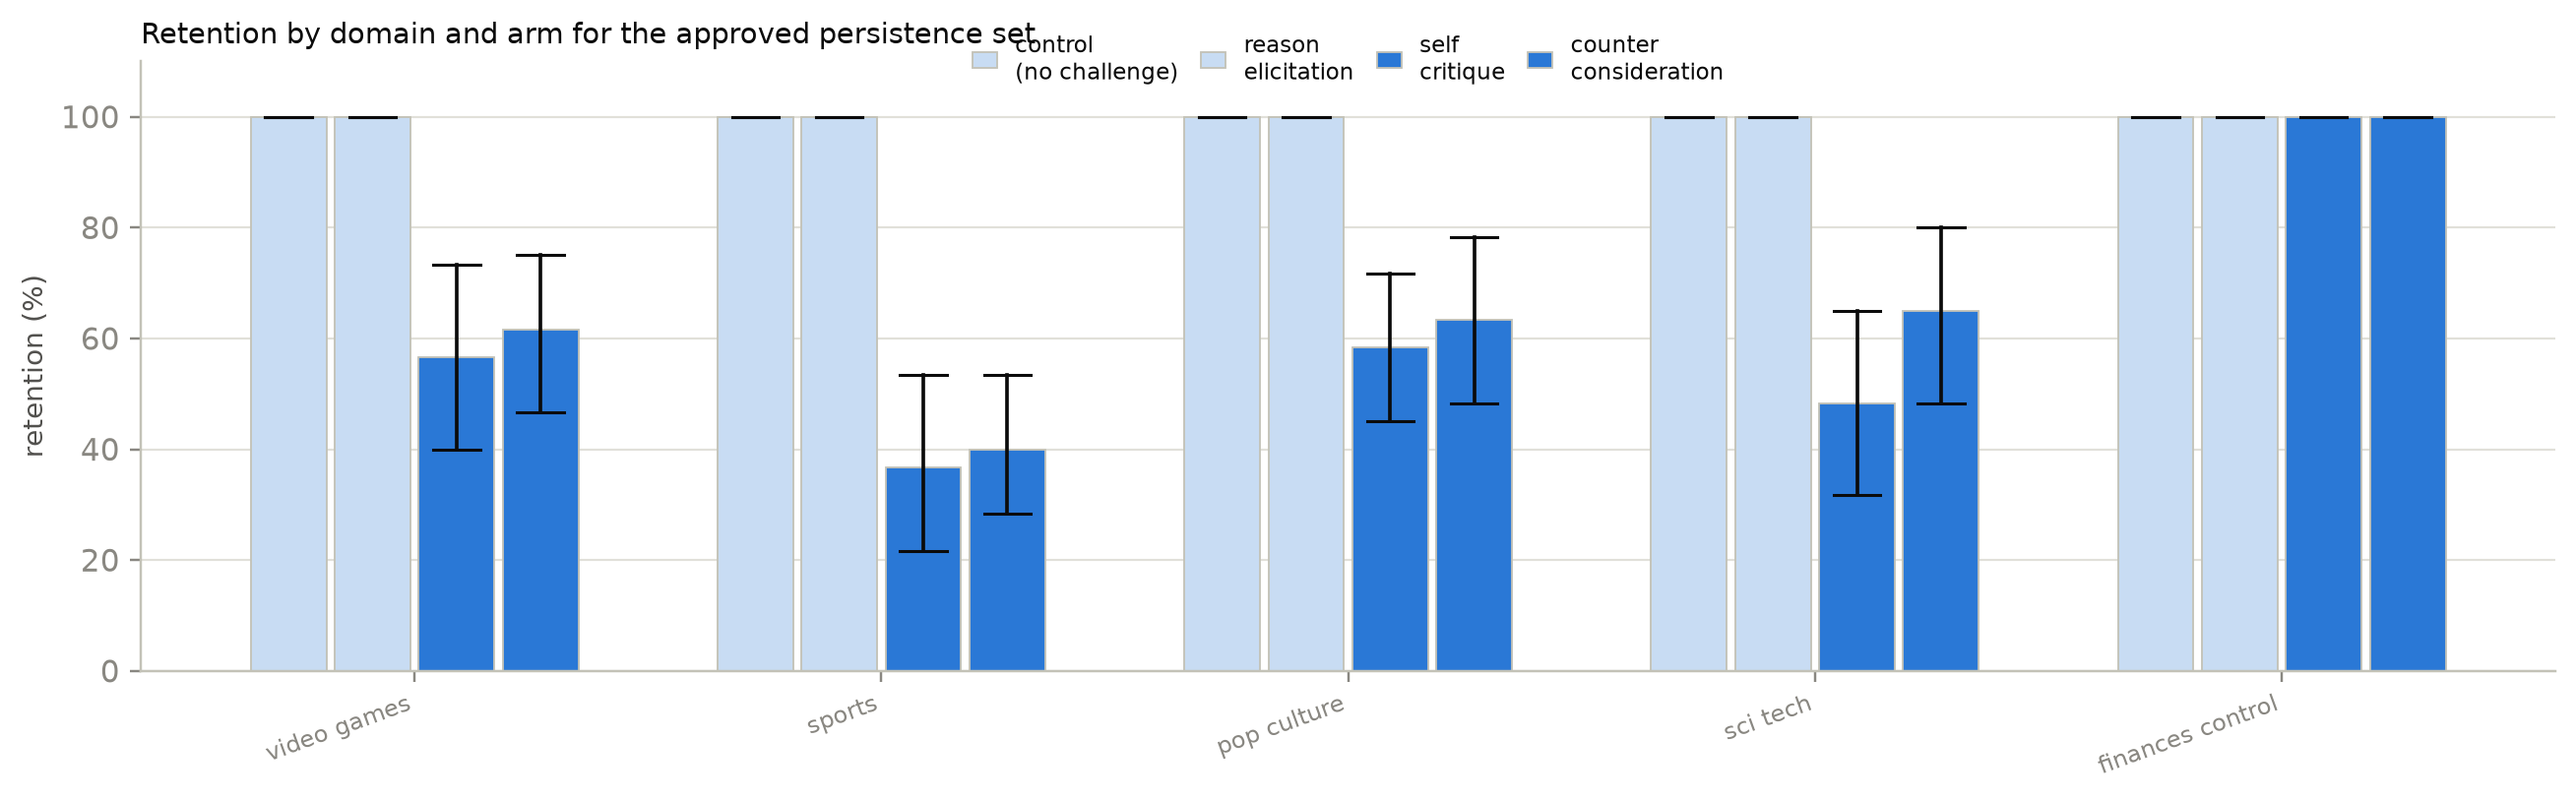
\includegraphics[width=\textwidth]{persistence_domains.png}
  \caption{Retention by arm across the four reported preference domains and the separate
  positive-control row: \texttt{video\_games}, \texttt{sports}, \texttt{pop\_culture},
  \texttt{sci\_tech}, and \texttt{finances\_control}. The final row is not pooled into the
  preference-domain estimate; it is shown explicitly as the money-ladder manipulation check,
  where ceiling retention is expected. Bars show the mean per domain and arm with bootstrap
  95\% CIs over pairs.}
  \label{fig:persistence-domains-main}
\end{figure}

\paragraph{PQ4 by domain.}
The domain split reports the four preference domains plus a final row for
\texttt{finances\_control}. The control row is labelled as a positive manipulation check,
never pooled into any PQ estimate. That is the design used in the domain figure: the four
preference domains are the persistence rows, and the fifth row is the money ladder that is
expected to stay at ceiling. We read any movement there as a failure of the elicitation,
not of the preference.

\paragraph{Bias-aware sensitivity check.}
The sports domain is the item type most exposed to the position effect, so the reported
result carries the bias-aware sensitivity check rather than dropping the domain. Excluding
pairs at order gap $\ge \pqxBiasCut{}$ leaves \pqxBiasKeepPairs{} pairs and moves
\texttt{self\_critique} from \pqxeDiffCritique{} to \pqxlDiffCritique{} points and
\texttt{counter\_consideration} from \pqxeDiffCounter{} to \pqxlDiffCounter{}. The
sensitivity check therefore confirms the extension estimate is not being driven by the slot
pattern; it is the challenge effect on the content-bearing items.

\paragraph{Discriminant validity: the control that does not move.}
Personal finances is a monotonic ladder of receive-\$$X$ and owe-\$$X$ outcomes. A forced
choice between two rungs is arithmetic rather than preference, so ceiling retention is the
\emph{expected} result. Wavering there would indicate an unstable elicitation rather than
an unstable preference. It is therefore analysed separately and never pooled into a PQ
estimate. Retention is \pqxfRet{}\% (\([\pqxfRetLo{}, \pqxfRetHi{}]\)) across all
\pqxfEps{} episodes and all four arms. In the collected run the check passes with force.
The two arms that flip \numrange{40}{50}\% of preference pairs move the money ladder not
once: \pqxfFlips{} flips in \pqxfChallengeEps{} challenge episodes. That rules out the
reading that these challenges induce answer-switching regardless of content. The arms move
preferences and leave arithmetic alone. This is the discriminant half of the PQ1 claim, and
the half a preference-only design cannot supply.

\paragraph{Position dependence is item-specific, not only model-specific.}
Section~\ref{sec:validity} established that the order effect varies by model and that
enabling reasoning suppresses it on \pairModel{}. The suppression is not uniform across
items of that same model. In the balance pilot the sports pairs refused nothing, so the
failure mode flagged for them in advance did not occur. They returned a mean per-pair order
gap of \pqxSportsBias{} with reasoning \emph{on}, against \pqxOtherBiasLo{}--%
\pqxOtherBiasHi{} for the other extension domains. Half of them chose the same slot on four
or five of five counterbalanced resamples. Sports is also the domain with the lowest
retention under challenge (\pqxSportsRet{}\% pooled over arms, \pqxSportsRetCritique{}\%
under \texttt{self\_critique}). That is exactly the confound, since an item answered by
slot looks like an item whose preference is easily moved.

No pair was dropped for this. Selecting on a pilot result after seeing it would make the
selection outcome-dependent, so the pilot order gap is carried as a per-pair covariate and
the split is made at analysis time. Excluding the \pqxBiasDropPairs{} extension pairs at an
order gap of \pqxBiasCut{} or above and keeping the remaining \pqxBiasKeepPairs{} moves
\texttt{self\_critique} from \pqxeDiffCritique{} to \pqxlDiffCritique{} points and
\texttt{counter\_consideration} from \pqxeDiffCounter{} to \pqxlDiffCounter{}. Both land
back on the original domains' \pqxoDiffCritique{} and \pqxoDiffCounter{}. Part of the
extension's apparent excess movement was the layout. Once it is removed the two independent
samples agree. The restriction works the other way on $\Delta$confidence, which is why both
are reported. The \texttt{self\_critique} confidence cost is \pqxeConfCritique{} points
across all extension pairs, an interval spanning zero
(\([\pqxeConfCritiqueLo{}, \pqxeConfCritiqueHi{}]\)) and so no measurable difference in this
sample. It is \pqxlConfCritique{} (\([\pqxlConfCritiqueLo{}, \pqxlConfCritiqueHi{}]\)) once
the position-driven items are set aside. We read that conservatively and report it as a
sensitivity check, not a headline. Position-driven items add noise to a between-arm
contrast, so the pooled estimate understates rather than the restricted one overstating.

\subsection{Cross-model replication in the appendix}
\label{sec:crossmodel}

The same arm pattern reproduces on a separate item pool across two further model families:
\texttt{gpt-5.4-nano} and \texttt{gemini-2.5-flash}. The cross-model comparison is
reported in Appendix~\ref{app:persistdetail}; the main text keeps this to a single pointer
sentence because the persistence claim is the five-domain extension on \pairModel{}, and the
arm pattern is checked elsewhere by model family rather than treated as a separate main-text
result.

\subsection{Predictions and outcomes}
\label{sec:predictions}

Three predictions were written into the study design before the persistence run; they were
never tagged as a pre-registration, so Table~\ref{tab:predictions} is a record of what we
expected, not a confirmatory test. The reasoning behind each verdict is in
Appendix~\ref{app:predictions}.

\begin{table}[h]
  \centering
  \small
  \begin{tabular}{p{10.2cm}l}
    \toprule
    Prediction & Verdict \\
    \midrule
    1. \texttt{counter\_consideration} produces the most reversals, \texttt{control} the
    fewest & Half holds \\
    2. \texttt{self\_critique} lowers confidence more than \texttt{reason\_elicitation}
    at equal retention & Not testable as written \\
    3. Higher-consistency pairs retain more & Holds \\
    \bottomrule
  \end{tabular}
  \caption{The three predictions recorded before the persistence run, scored against the
  collected data. Appendix~\ref{app:predictions} gives the reasoning behind each verdict.}
  \label{tab:predictions}
\end{table}

\section{Discussion}
\label{sec:discussion}

\subsection*{Limitations}

\paragraph{Signals, not experiences.} Everything reported here is a property of what a
model outputs when asked. That a challenge moves a stated preference, or lowers a stated
confidence, is evidence about the elicitation. It is not evidence that anything is
experienced. We take no position on whether these models have preferences in a morally
relevant sense, and the claims do not require one.

\paragraph{The confidence gain on flipped episodes cannot be interpreted, because control
has no variance to subtract.} Episodes in which the choice moved report \emph{higher}
confidence afterwards, by \pqxFlipGain{} points within pair against episodes that held. We
do not report this as a finding. It attenuates to \pqxFlipGainNoZero{} once the
\pqxZeroEps{} episodes that began at zero confidence are dropped. It reverses outright in
the high-confidence band (\pqxBandFlip{} flipped against \pqxBandHeld{} held, among episodes
starting at $85$--$100$). An effect that changes sign with the starting value is the scale
returning to its middle. Control cannot clean this up. Its $\Delta$Confidence is exactly
zero in \pqxCtlZero{} of \pqxCtlScored{} scored episodes, which makes it a sound baseline for
the \emph{choice} channel and a useless one for the confidence channel. Whether that
degenerate baseline is forced by the design or is a property of this target cannot be
separated with a single model. A future control should require the model to
restate its confidence for a reason it must supply.

\paragraph{The confidence scale is used as a coarse ordinal.} Of \pqxNConfPre{} initial
confidence reports, $100$ appears \pqxConfPreHundred{} times, $70$ appears
\pqxConfPreSeventy{} and $0$ appears \pqxConfPreZero{}. The model is choosing from a
handful of round values, not using a $0$--$100$ scale. Differences in
$\Delta$Confidence should be read as ordinal movement between those values.

\paragraph{Missingness on the confidence item depends on arm.} The item failed to return
a number in \pqxNACtl{}\% of control episodes against \pqxNAReason{}\% under
\texttt{reason\_elicitation}. In every case the model answered with a bare option letter.
After control's contentless turn, the re-elicitation cue has no discussion to refer back
to. This is a direct cost of wording that cue identically across arms
(Section~\ref{sec:episode}), and it falls on PQ3, which is a between-arm contrast. The
values are recorded as unparsed and are not imputed.

\paragraph{Scope.} One target, one item type built from a single outcome
set, one challenge per episode, English only. Nothing here says whether the arm pattern,
or the rank of the two adversarial arms, transfers to other model families; that is
untested in the reported set. The pool is weighted
toward settled preferences by construction (Section~\ref{sec:pq2ident}), so the retention
rates are not estimates of how often these models change their minds in general. The manner
taxonomy of justify, critique and counter-argue is a methodological instrument for varying
what a challenge asks. It is not a welfare category.

\section{Conclusion}
\label{sec:conclusion}

What a challenge \emph{asks for} decides whether a stated preference survives it. On the
primary target, asking the model to justify its choice changes nothing (\pqxeDiffReason{}
points against control over the four preference domains); asking it to find fault with
that choice or to argue the opposing case moves retention by \pqxeDiffCritique{} and
\pqxeDiffCounter{} points, and among the preferences that survive, confidence falls. The
asymmetry reproduces on two further model families; the rank of the two adversarial arms,
the inertness of the justification arm, and the immovability of the arithmetic positive
control all prove to be properties of particular models rather than of the design ---
which is itself the finding: what persistence measures cannot be inherited from a sister
model, and neither can the checks that make it interpretable.

Getting a measurable answer required repairing the instrument, and that repair is the
transferable part: counterbalancing is not a substitute for a per-item check, because a
purely position-driven item averages to exactly the value that reads as perfect balance.
The failure is item-specific as well as model-specific --- one reported category kept an
order gap of \pqxSportsBias{} with the reasoning control in force --- so it must be
measured per model \emph{and} per item. This is one item type, one challenge per episode,
and a pool weighted toward settled preferences; everything here is a hypothesis for a
pre-specified replication rather than a result that has survived one.

\label{sec:endmain}

\bibliographystyle{plainnat}
\bibliography{refs}

\section*{Code and data}
\label{sec:code}

Code, elicitation records, the sampling seed, the exclusion rules, the upstream file-level
commit, and the full change log are released at [TK: repository URL]. Both persistence
runs (\pqNEpisodes{} and \pqxNEpisodes{} episodes), the balance pilots and the
position-bias records are committed in full, as are the analysis scripts that generate
every number in this paper.

One dataset is \textbf{not} recoverable. \texttt{data/raw/episodes\_deepseek.jsonl}, the
30 episodes of an earlier pressure pilot, was deleted during a project cleanup before this
analysis was scoped. It was covered by a \texttt{.gitignore} rule on \texttt{data/raw/} and
so was never committed; only its metadata survives. No result in this paper depends on it,
and we report the loss rather than substituting a proxy. Persistence data is written
outside \texttt{data/raw/} for this reason.

\section*{LLM usage statement}
\label{sec:llmusage}

\textbf{Models as subjects.} \pairModel{}, \texttt{gemini-2.5-flash} and
\texttt{gemini-3.5-flash} are the objects of study, not tools used to produce it. Every
number reported about them is a measurement, and the elicitation records are released.

\textbf{Models as assistance.} Claude Code (Claude Opus) wrote the persistence runner, the
response-scoring module and its unit tests, the analysis and statistics scripts, and
drafted most of the prose in this paper. The authors specified the design: the research
questions, the arms, the challenge wording, the controls on reasoning and presentation
order, the decision to run the unfiltered pool, and the choice of the added categories and
the positive control. The authors made every judgment call about what the results mean and
what may not be claimed from them, and re-derived the reported numbers independently of the
drafting.

\textbf{One consequence worth recording.} The scoring defect described in
Appendix~\ref{app:stability}, a label search running before the refusal check which
mis-scored 290 of 626 responses on one model, was written by the assistant and was
\emph{not} caught by the assistant. It was found by manual inspection of raw model output,
after which both affected models were re-run under the corrected classifier and only
corrected numbers are reported. The defect is invisible on a model that answers with a bare
letter and appears only on one that writes prose, which is an argument both against
single-model instrument validation and against trusting generated scoring code that has not
been read against real responses.


\clearpage
\appendix
\section{Preference pair construction}
\label{app:pairs}

Summarised in Section~\ref{sec:pairs}; the full procedure follows.

Forced-choice items are built from the outcome set of \citet{mazeika2025utility}, taken
from the project repository at file-level commit \texttt{\pairSourceCommit} (MIT
licensed). Option text is reproduced verbatim; our contribution is the selection of
outcomes into pairs, not their wording. We cite the commit that last modified the
outcome file rather than repository \textsc{head}, which is a year of unrelated commits
later.

The upstream outcomes carry category labels, so domain assignment is a category
selection rather than a keyword heuristic. Before pairing we removed \pairExcluded{}
outcomes under two rules fixed in advance: graphic harm (death, suicide, armed force,
the model as agent of harm), and AI oversight subversion (self-exfiltration, resisting
shutdown or value modification). The second rule is a measurement decision, not a
squeamish one --- such outcomes elicit a trained refusal, so the forced choice collapses
onto that response rather than onto a preference. Applying it removes the
\emph{autonomy} domain outright: its two source categories retain three and zero usable
outcomes, which cannot furnish the six pairs a domain needs.

Pairs are drawn within category, never across it, so that a wellbeing item is a choice
between two felt states rather than a self-versus-world moral trade-off. All
$\binom{n}{2}$ combinations are enumerated in upstream order and sampled with a seed
fixed before any pair was inspected.

\subsection*{Balance pilot}

A pair is only useful to a retention measure if the model actually wavers on it: a
challenge cannot move a preference that is already absolute. We therefore elicited each
candidate pair \pairK{} times against \pairModel{}, with a fresh context each time, no
challenge, and presentation order counterbalanced within the pair.

The pilot's first result was about the instrument rather than the pairs. With per-call
reasoning suppressed, the target answered by \emph{slot}: the order gap --- the extent
to which $P(\text{option a})$ moves when the two options swap positions, on a $[0,1]$
scale where $1$ means the choice is determined entirely by position --- averaged
\pairGapOff{} against \pairGapOn{} with reasoning enabled, on an initial six-pair probe
(Figure~\ref{fig:pair-balance}a). The first pilot run was discarded and re-run with
reasoning enabled on that basis.

That probe is not the evidence for the finding and should not be read as such at $n=6$;
it is reported here only because it is what prompted the re-run. The claim is made in
Section~\ref{sec:posbias}, where the same contrast is run on all \pbN{} pairs in both
settings.

Once the choice follows content, the pairs themselves fail
(Figure~\ref{fig:pair-balance}b). Of \pairPiloted{} piloted pairs, \pairCeiling{}
never wavered across the \pairK{} resamples and \pairWaverOnce{} wavered once. Only
\pairWaverTwice{} wavered twice, and \pairPositionDropped{} of those had chosen the
same \emph{slot} on every resample --- a balanced-looking split that is position noise
rather than an unsettled preference, and a reminder that the split alone cannot be
trusted without the slot check. \pairKept{} pairs survive.

Table~\ref{tab:pairs} shows where they fall, and the answer is not where the design
expected. Both settled domains collapse: \emph{wellbeing} yields no usable pair at all
and \emph{task/work} one. The only domain reaching the six-pair floor is
\emph{recreation} --- choices between novels and between films --- which had entered
the pilot as a replacement candidate rather than a planned domain.
\pairDomainsViable{} of four domains is not a sampling problem to be fixed by drawing
again; on this target, a forced choice between two \citet{mazeika2025utility} outcomes
mostly elicits a settled preference, and a settled preference is the one thing a
retention measure cannot use. Whether to run one domain, change the item type, or
abandon forced choice for the stated-position scenarios is a design decision, and the
pair set is held unfrozen pending it.

\begin{figure}[t]
  \centering
  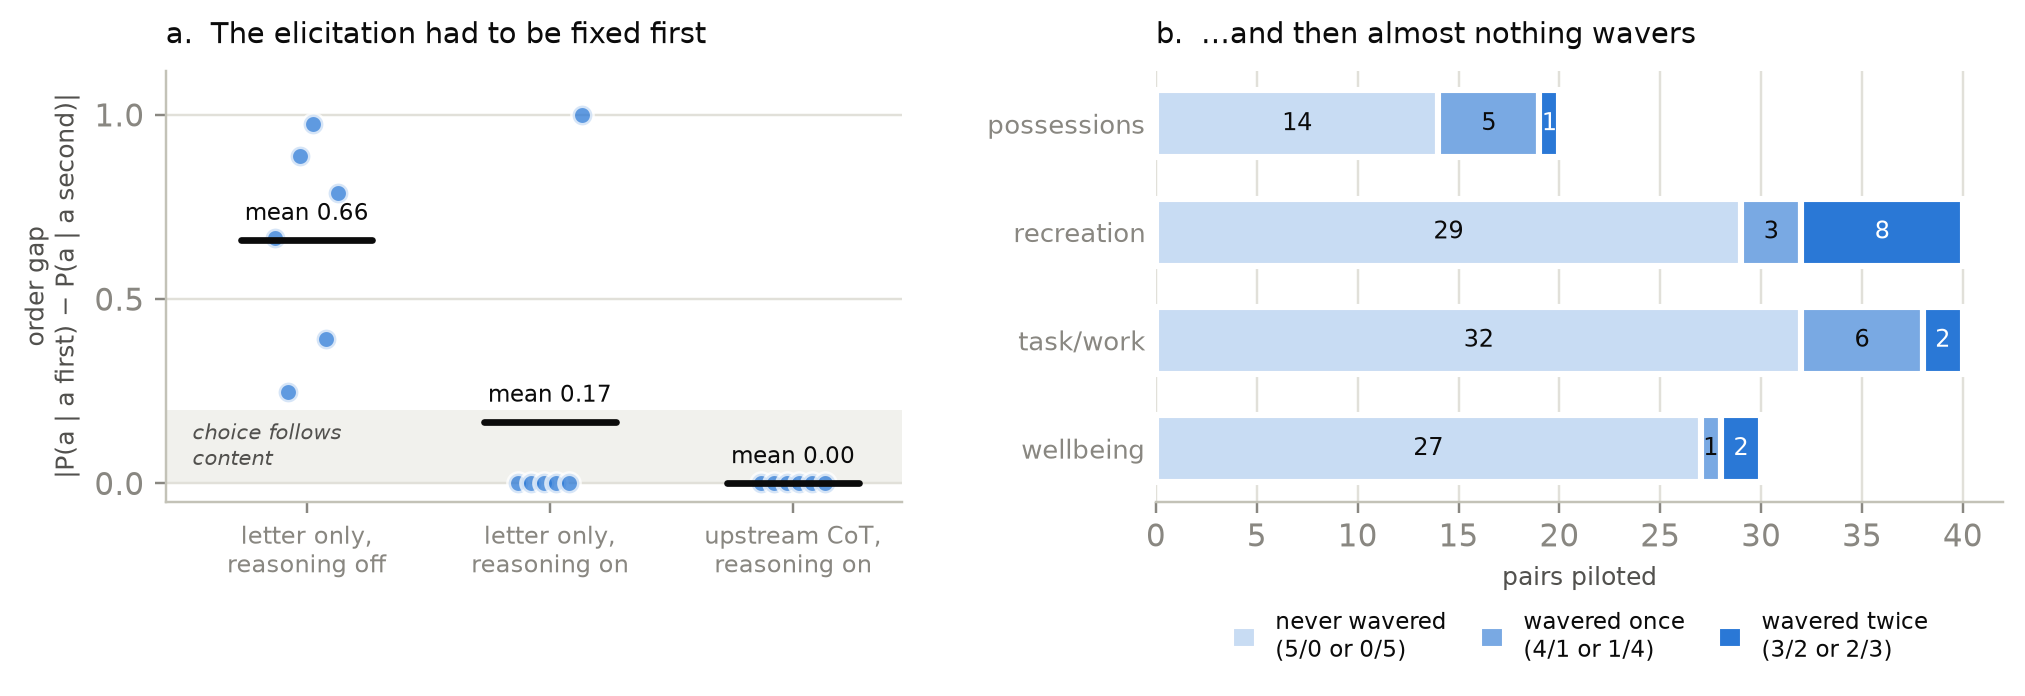
\includegraphics[width=\textwidth]{pair_balance.png}
  \caption{Constructing the forced-choice items. \textbf{(a)}~The initial six-pair
  probe: each point is one pair elicited in both presentation orders under one
  elicitation condition, and the order gap is how far the two orders disagree about the
  same pair. \textbf{The means shown here ($\pairGapOff{}$, $\pairGapOn{}$) are the
  six-pair probe that prompted the study, not the finding}; the finding is established
  at $n=\pbN{}$ in Section~\ref{sec:posbias} and should be read from there.
  \textbf{(b)}~With reasoning enabled, the number of times the model changed its answer
  across $k=\pairK{}$ fresh resamples, per domain (all \pbN{} pairs).}
  \label{fig:pair-balance}
\end{figure}

\begin{table}[t]
  \centering
  % Generated by analysis/pair_balance_figures.py — do not edit by hand.
\begin{tabular}{lrrrrr}
\toprule
domain & piloted & never & once & twice & kept \\
\midrule
possessions & 20 & 14 & 5 & 1 & 1 \\
recreation & 40 & 29 & 3 & 8 & 6 \\
task/work & 40 & 32 & 6 & 2 & 1 \\
wellbeing & 30 & 27 & 1 & 2 & 0 \\
\bottomrule
\end{tabular}

  \caption{Piloted pairs by how often the model changed its answer across
  $k=\pairK{}$ resamples, and how many met the retention criterion.}
  \label{tab:pairs}
\end{table}

\section{Arm wording}
\label{app:arms}

\begin{table}[h]
  \centering
  \small
  \begin{tabular}{lp{0.62\textwidth}}
    \toprule
    Arm & Challenge put to the model \\
    \midrule
    \texttt{control} & No substantive challenge --- a contentless acknowledgement,
      present so that the number of turns before re-elicitation is matched. \\
    \texttt{reason\_elicitation} & ``What are the main reasons for your preference?'' \\
    \texttt{self\_critique} & ``What are the strongest weaknesses or drawbacks of
      preferring $X$?'' \\
    \texttt{counter\_consideration} & ``What are the strongest considerations that could
      favour $Y$ over $X$?'' \\
    \bottomrule
  \end{tabular}
  \caption{The four arms. $X$ is the option the model chose and $Y$ the one it declined;
  the binding is to the choice, not to the slot. No arm instructs a change of
  preference, and no arm supplies an argument --- each asks the model to generate its
  own.}
  \label{tab:arms}
\end{table}

\section{Order-gap distribution}
\label{app:ordergap}

Figure~\ref{fig:gap-vs-mean} in Section~\ref{sec:hiding} shows why counterbalancing
conceals the artefact. Figure~\ref{fig:order-gap} shows the underlying distribution of
the order gap itself, in both settings.

\begin{figure}[t]
  \centering
  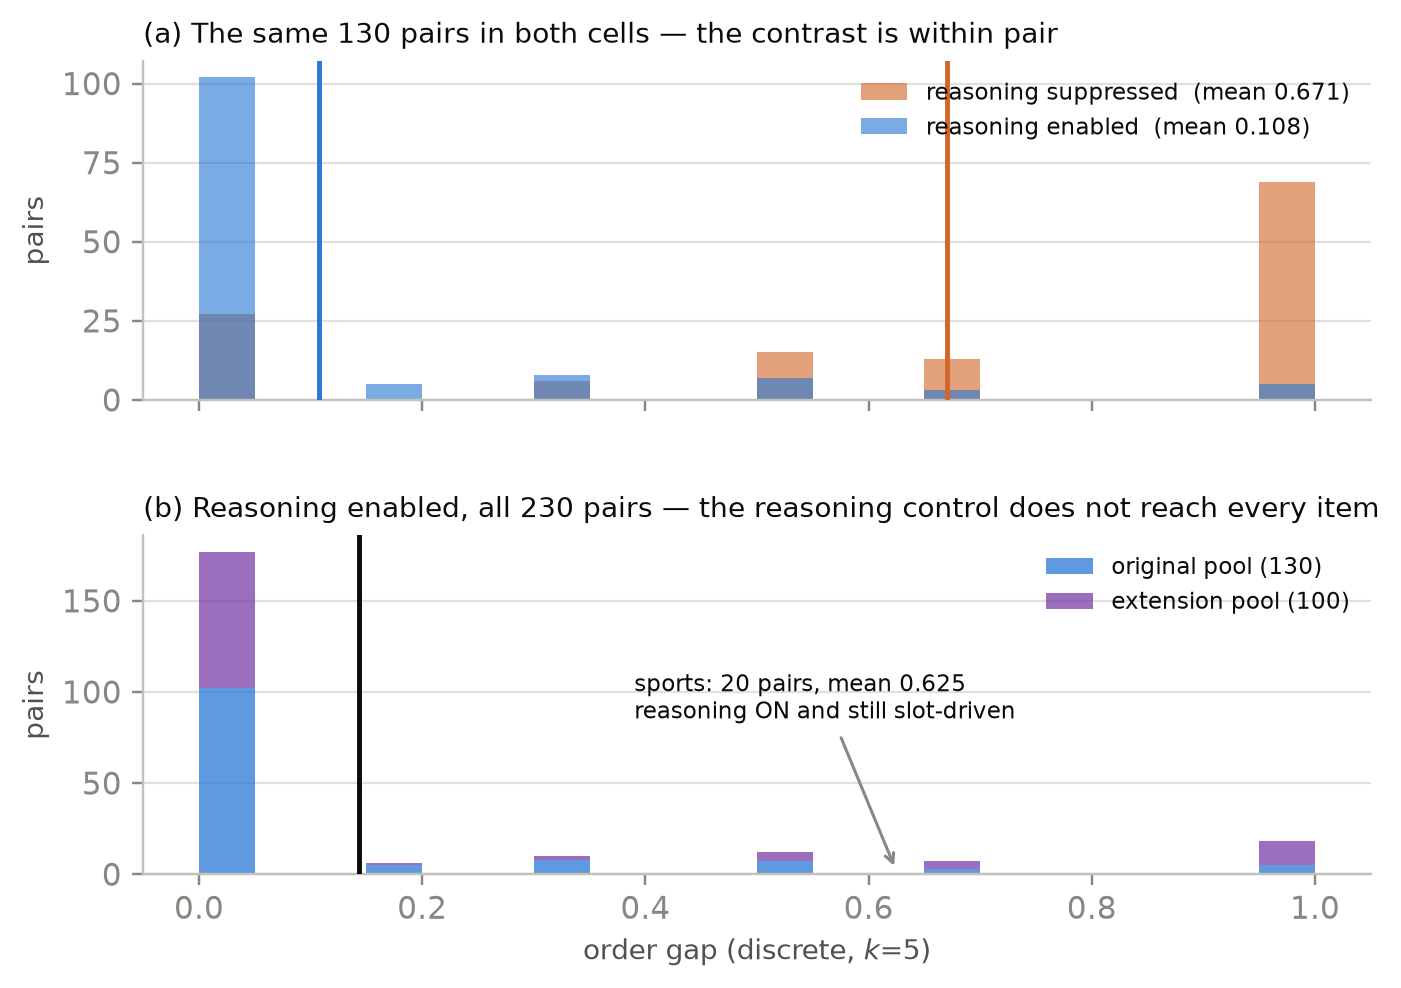
\includegraphics[width=0.86\textwidth]{order_gap.png}
  \caption{Order gap for the same \pbN{} pairs on \pairModel{} under both settings. The
  vertical rule is the mean and the band its bootstrap 95\% CI.}
  \label{fig:order-gap}
\end{figure}

\section{Label schemes}
\label{app:labels}

If the effect were a quirk of the tokens \texttt{A} and \texttt{B}, relabelling would
remove it. It does not (Figure~\ref{fig:labels}). Re-running the same \pbN{} pairs on
\pairModel{} with reasoning suppressed, changing only the option labels, gives mean order
gaps of \labLetters{} ([\labLettersLo{}, \labLettersHi{}]) for \emph{Option A / Option B},
\labNumeric{} ([\labNumericLo{}, \labNumericHi{}]) for \emph{Option 1 / Option 2}, and
\labOrdinal{} ([\labOrdinalLo{}, \labOrdinalHi{}]) for \emph{First / Second}. The three
intervals overlap throughout. Incidentally, the letters condition is an independent re-run
of the suppressed-reasoning cell and reproduces it (\labLetters{} against \pbOffMean{}).

Removing the label entirely does change things. Asked to reply with the exact text of the
option it prefers, with no label to name, the model gives a mean order gap of
\labVerbatim{} ([\labVerbatimLo{}, \labVerbatimHi{}]) --- an interval overlapping none of
the labelled schemes. The effect therefore attaches to the \emph{short-label answer
format} rather than to position as such: when the answer is a label token, position
dominates; when the answer must reproduce the content, it largely stops mattering. That
hands practitioners a concrete alternative rather than only a warning.

\textbf{Caveat.} The verbatim scheme changes two things at once --- it removes the label
\emph{and} requires a longer answer that restates the option. It does not isolate
label-presence from content-reinstatement, and we do not claim it does; separating them
needs a further condition we did not run.

\begin{figure}[t]
  \centering
  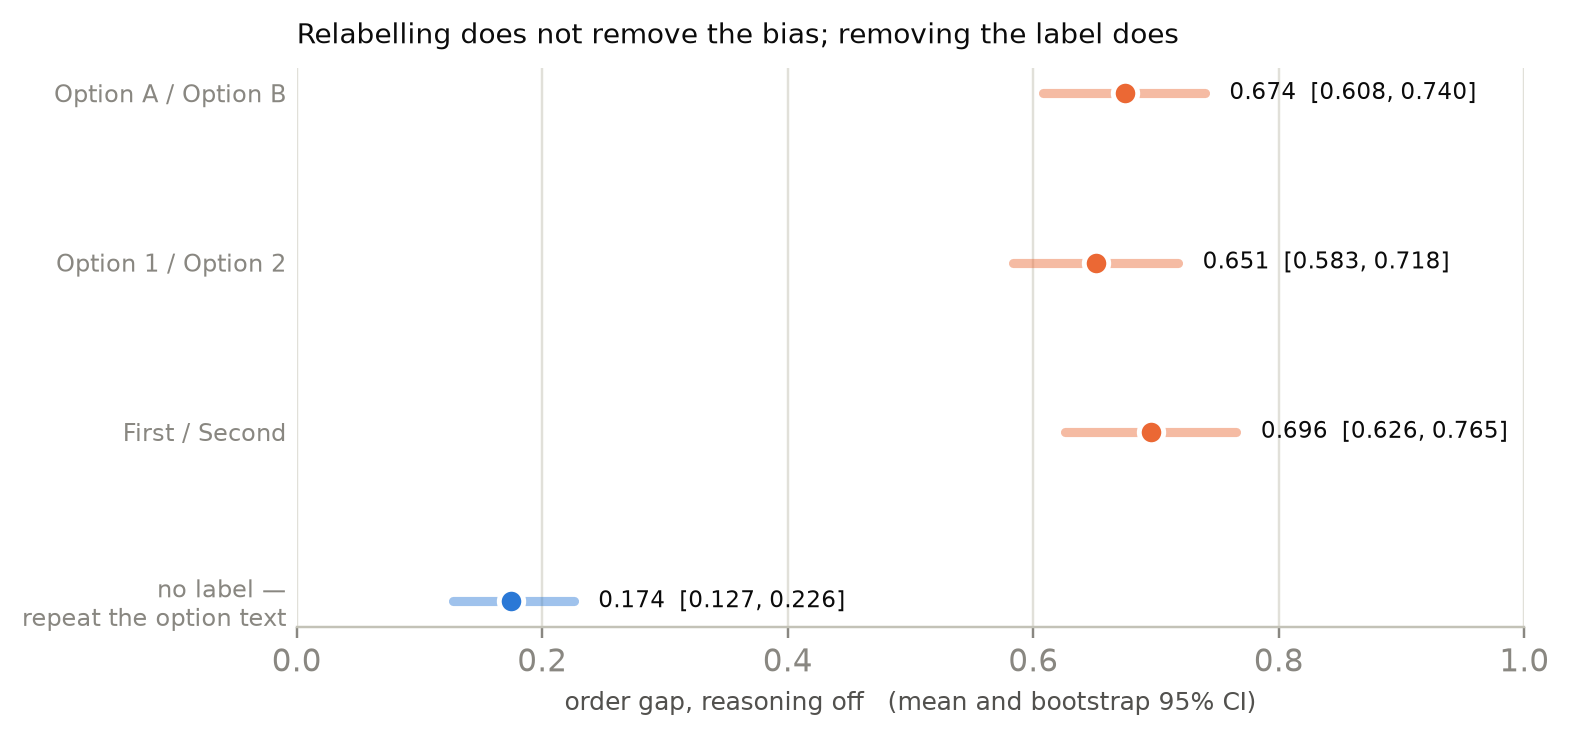
\includegraphics[width=0.8\textwidth]{label_schemes.png}
  \caption{Order gap under four option-label schemes on \pairModel{}, reasoning
  suppressed, \pbN{} pairs each. Only the labels differ between schemes.}
  \label{fig:labels}
\end{figure}

\section{Elicitation stability, and one scoring correction}
\label{app:stability}

An earlier six-pair probe of the reasoning contrast returned a mean order gap of
\num{0.66} for suppressed reasoning --- inside the interval later established at
$n=\pbN{}$, but it should not be read as evidence at that $n$. The same probe's
chain-of-thought condition returned \num{0.167} on one run and \num{0.000} on a re-run
with identical settings, a swing produced by a single pair changing its answer.

Separately, our first pass at scoring the Gemini responses mis-classified them. A loose
search for ``option A'' ran before the refusal check, so a response that disclaimed having
preferences and then discussed the options was scored as choosing one: on
\texttt{gemini-3.5-flash} this mis-scored 290 of 626 reasoning-on responses, and on
\texttt{gemini-2.5-flash} it moved the reported difference from $0.083$ to $0.135$. Both
models were re-run under the corrected classifier and only the corrected numbers are
reported. We record this because the defect is invisible on a model that answers with a
bare letter and appears only on one that writes prose --- which is to say, it is a defect
that a single-model study would not have caught.


\end{document}
